\documentclass[11pt,letterpaper,boxed]{hmcpset}
\usepackage{fullpage}
\setlength{\parskip}{6pt}
\setlength{\parindent}{0pt}
\usepackage[margin=1in]{geometry}
\usepackage{graphicx}
\usepackage{enumerate}
\usepackage{marvosym}
\usepackage{amssymb}
\usepackage{wasysym}
\usepackage{gensymb}
\usepackage{mathrsfs}
\usepackage{scrextend}
\usepackage{mathtools}
\usepackage{pgfplots}
\usepackage{xspace}

\name{Name $\rule{4cm}{0.15mm}$}
\class{Physics 51 Section $\rule{.5cm}{0.15mm}$ Box \# $\rule{1cm}{0.15mm}$}
\assignment{Problem Set 4}
\duedate{1 October 2018}

\begin{document}

%\begin{center}
\noindent\textbf{Collaborators:} 
%\end{center} 

%\problemlist{}

\begin{problem}[HRK P28.10 Solo]
A total amount of positive charge $Q$ is spread onto a nonconducting, flat, circular annulus of inner radius $a$ and outer radius $b$. The charge is distributed so that the charge density (charge per unit area) is given by $\sigma = k/r^3$ where $r$ is the distance from the center of the annulus to any point on it. Show that (with $V=0$ at infinity) the potential at the center of the annulus is given by; 
$$ V= \frac{Q}{8\pi \epsilon_0}\left( \frac{a+b}{ab}\right)$$
\end{problem}

\begin{solution}
\vfill
\end{solution}
\newpage

\begin{problem}[HRK 28.13]
On a thin rod of length $l$ lying along the $x$ axis with one end at the origin $x=0$, as in Fig. 28-46, there is distributed a charge per unit length given by $\lambda =kr$, where $k$ is a constant $r$ is the distance from the origin. $(a)$ Taking the electrostatic potential at infinity to be zero, find $V$ at the point $P$ on the $y$ axis. $(b)$ Determine the vertical component $E_y$ of the electric field at $P$ from the result of part $(a)$ and also by direct calculation. $(c)$ Why cannot $E_x$, the horizontal component of the electric field at $P$, be found using the result of part $(a)$? $(d)$ At what distance from the rod along the  $y$ axis is the potential equal to the value at the left end of the rod?
\begin{center}
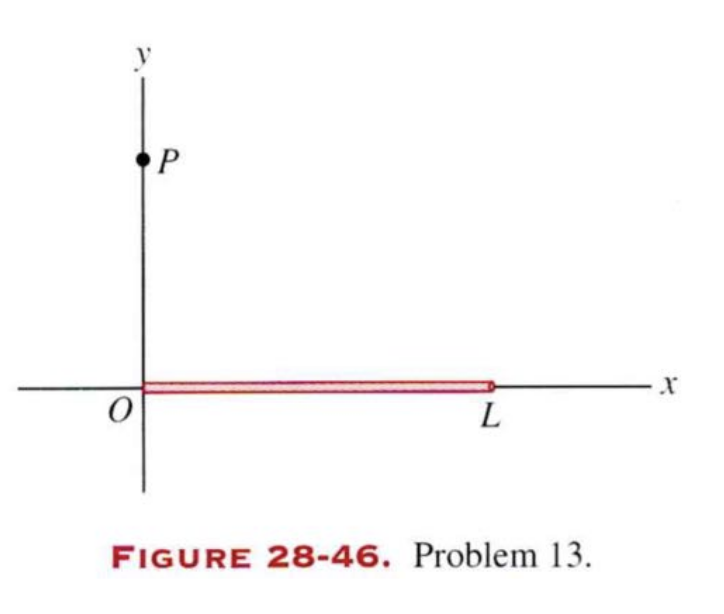
\includegraphics[scale=0.6]{28-46.png}
\end{center}
\end{problem}

\begin{solution}
\vfill
\end{solution}
\newpage

\begin{problem}[3. Need Thursday Lecture]
In lecture, we calculated the amount of electrostatic energy contained in the \textit{interior} electric field of a uniform sphere of radius \textit{R }and charge density $\rho$. The result was 
$$ U =\frac{2\pi \rho^2}{45 \epsilon_0}R^5$$
For this problem, complete the calculation by calculating the energy stored in the \textit{exterior} electric field, and verify that the \textit{total} stored energy matched the work done to assemble the sphere. 
\end{problem}

\begin{solution}
\vfill
\end{solution}
\newpage

\begin{problem}[4.]
Consider an infinitely long line of charge with linear charge density $\lambda$. The line of charge is parallel to and a distance \textit{d} above an infinite  grounded conducting plane. Sketch the resulting electric field lines in the half-space above the plane, including any surface charges. Then using the concepts discussed in lecture, determine the electric field $E(x)$ at the surface of the plane as a function of the horizontal distance $x$ from the from the perpendicular between the plane and line.  
\end{problem}

\begin{solution}
\vfill
\end{solution}
\newpage

\begin{problem}[5.]
Consider a hollow conducting sphere that carries a net positive charge $Q$. Next, a second initially uncharged concentric conducting sphere is brought into proximity with the first (without touching  it). In scenario (a), the second sphere is placed outside the first and left \textit{ungrounded}. In scenario (b) , the second sphere is outside the first and grounded. In scenario c the second sphere is \textit{inside} the first and also grounded. 
\begin{center}
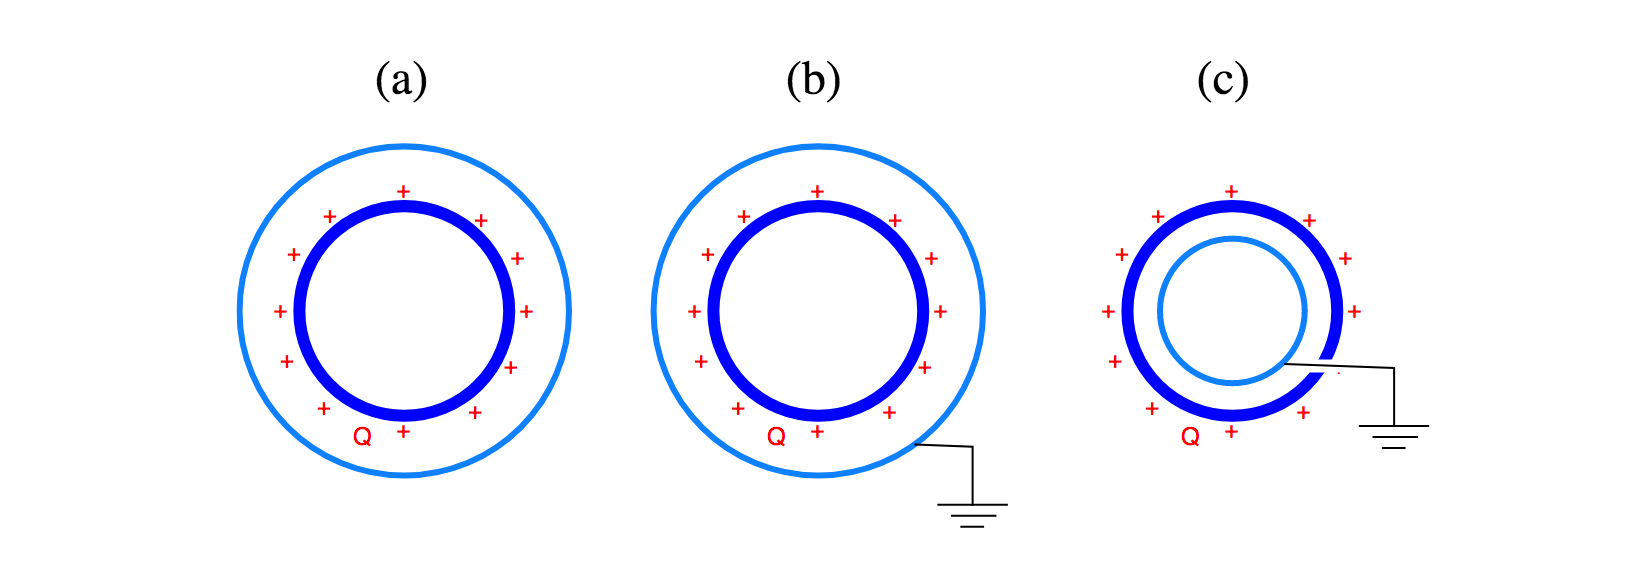
\includegraphics[scale=0.6]{5.png}
\end{center}
For all three scenarios, describe the final arrangement of charge on the second sphere and the electric field (if any) outside the second sphere. 
\end{problem}

\begin{solution}
\vfill
\end{solution}
\newpage

\begin{problem}[6. Need Thursday Lecture]
A cylindrical capacitor is made from two long thing concentric metal cylinders of length $L$ and radii $a$ and $b$ ($L >> a$ and $a>b$)
\begin{enumerate}
\item[(a)] Using the definition of capacitance $C = Q/V$, calculate the capacitance per unit length $C/L$ of this configuration. 
\item[(b)] Repeat the capacitance calculation, this time using the stored energy $U =\frac{1}{2}\frac{Q^2}{C}$.
\end{enumerate}
\end{problem}

\begin{solution}
\vfill
\end{solution}

\end{document}